\documentclass[twocolumn]{article}

%\usepackage{cleveref}
\usepackage{amsmath}
\usepackage{float}
\usepackage{graphicx}
\usepackage{caption}
\usepackage{subcaption}


% Make table names in captions boldfaced
\captionsetup[table]{labelfont=bf}
\captionsetup[figure]{labelfont=bf}

\begin{document}
%opening
\title{The radio blackout effect of plasma sheaths at hypersonic and reentry velocities}
\author{Jack Nelson,\\
	Physics Department,\\
	Occidental College, Los Angeles, CA}
\date{October 2016}
\twocolumn[ % hacky trick to get a one-column abstract in a two-column article
	\begin{@twocolumnfalse}
		\maketitle
			\begin{abstract}
			 Airborne vehicles traveling through an atmosphere at hypersonic velocities, especially in excess of Mach 15, face significant atmospheric heating that produces a plasma sheath which surrounds the vehicle.
			 Depending on the density of the atmosphere, the shape of the vehicle, and its speed, free electrons in the plasma attenuate and reflect incident electromagnetic waves, making communication to and from the hypersonic vehicle difficult or impossible.
			 Various methods of communicating through the plasma sheath have been proposed and studied since the early 1960's, yet a single elegant solution has not been found in unclassified research to date.
			 
			 In this paper, we will establish a theoretical framework of the problem and look at the associated plasma physics in order to better contextualize the potential solutions.
			 These solutions can be divided into two basic types: passive methods, which minimize blackout conditions through the vehicle or mission design, and active methods, which use active systems to change or exploit the properties of the plasma flow field to communicate through the plasma barrier.
			 We will examine some of the passive and active solutions that have been proposed, as well as recent studies of active electromagnetic fields and $\mathbf{E}\times\mathbf{B}$ Lorentz forces.
			 A method which uses scattered Stokes waves and Raman interactions of an electromagnetic ``pump" wave with resonances in the plasma sheath induced by external radio waves is presented as a solution that has the potential to minimize weight and equipment volume in the vehicle, yet remain effective.
	 
	
			\end{abstract}
		\end{@twocolumnfalse}
	]
\section{Introduction}
	Spacecraft reentering an atmosphere from orbit and aircraft traveling at hypersonic speeds experience the problem of aerodynamic heating, in which their large kinetic energies are transferred into heat by hypersonic interactions with the atmosphere.
	The problem of convective aerodynamic heating of a reentry vehicle was adequately solved by the time of the first human space flights in the early 1960's.
	For reentry speeds, it was found that blunt bodies as opposed to slender, streamlined ones minimize the total heat transferred to the vehicle from the air.\cite{allen_study_1958}
	Blunt body capsule designs, coupled with ablative heat shield technology, created a simple yet effective solution to the reentry heating problem which is still widely used today.
	
	For hypersonic aircraft which operate at less than reentry speeds, such as NASA's X-15 piloted research vehicle, the heating problem is solved using thick skin heat sinks made of high heat capacity superalloys such as Inconel-X.\cite{stillwell_x-15_1965}
	
	A side-effect of the hypersonic heating problem is the generation of plasmisized atmospheric gases and the formation of a plasma sheath which envelopes the vehicle.
	The electromagnetic properties of the plasma sheath result in attenuation and reflection of incident radio waves, depending on the frequency of the wave and the density of the plasma.
	As a result, reentering spacecraft and high-hypersonic aircraft surrounded by dense plasma sheaths will enter periods of radio blackout where normal radio communication is completely blocked by the plasma.
	Figure \ref{fig:RAMCBlackout} shows a typical blackout profile of radio signals of different frequencies over altitude and speed for a low Earth orbit (LEO) spacecraft reentry.
	
	\begin{figure}[h]
		\centering
		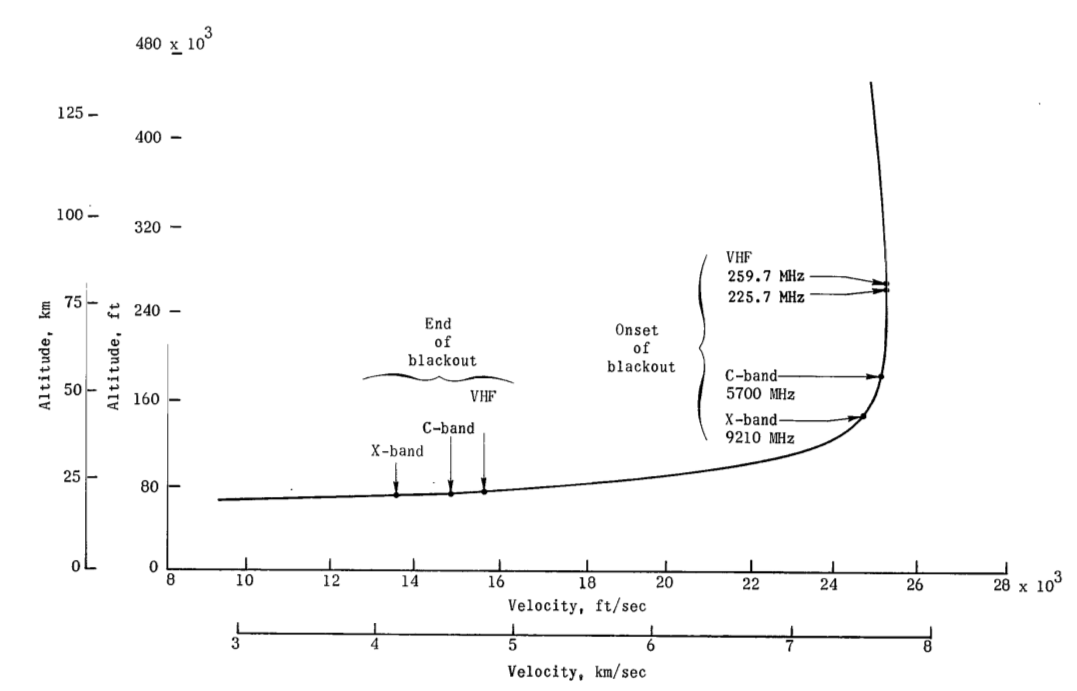
\includegraphics[width = 0.5\textwidth]{Images/RAMC_BlackoutProfile.png}
		\caption{\textbf{The blackout profiles of VHF, C-band, and X-band radios over altitude and velocity during the RAM C-1 reentry. Figure 10 from \cite{akey_radio_1970}.}}
		\label{fig:RAMCBlackout}
	\end{figure}
	
	An overview of the paper is as follows: section \ref{sec:PlasmaSheaths} summarizes the basic properties of hypersonic vehicle plasma sheaths and introduces the plasma frequency $\omega_p$ as a fundamental measure of whether a plasma sheath will attenuate a radio wave with carrier frequency $\omega$.
	Section \ref{sec:Waves} gives an overview of electromagnetic waves propagating through a plasma, as well as waves in the plasma medium itself, referred to as Langmuir waves or electron acoustic waves.
	In section \ref{sec:Overview}, a number of promising solutions to the blackout problem are divided into active and passive methods, and each method is summarized and evaluated.
	
\section{Plasma Sheaths of Hypersonic Vehicles} \label{sec:PlasmaSheaths}
In this section, we will summarize the processes by which plasma is generated by a hypersonic vehicle, as well as the characteristic properties of the plasma.
This theory, combined with the additional theory of waves in plasmas presented in section \ref{sec:Waves}, will provide a theoretical basis to understand and evaluate solutions to the radio blackout problem.

Vehicles traveling through an atmosphere at speeds greater than Mach 5 create strong shock waves in front of them which generates varying amounts of plasma from atmospheric gases.
The generation of this plasma, and its enveloping of the entire vehicle in a sheath, is what prevents radio signals from reaching or leaving the vehicle.
As a critically important problem that needed to be solved for both ballistic missile reentry vehicles and crewed spacecraft, the aerodynamic shock heating problem has been studied extensively since the 1950's.\cite{allen_study_1958}\cite{dunn_theoretical_1973}\cite{allen_aerodynamic_1964}\cite{launius_coming_2012}.

\begin{figure*}[t]
	\centering
	\begin{subfigure}{0.5\textwidth}
		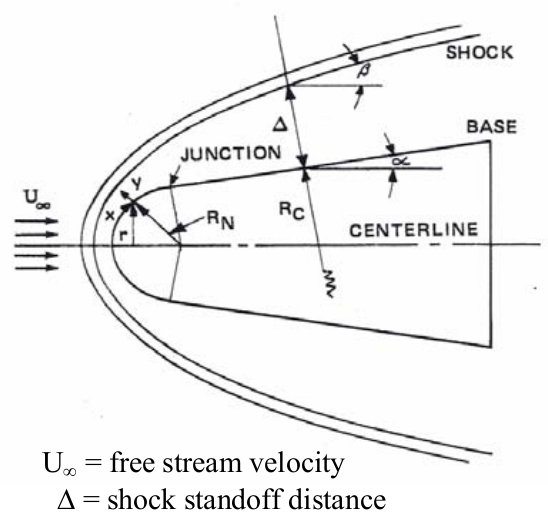
\includegraphics[width = 0.8\textwidth]{Images/BluntBody.png}
		\caption{\textbf{A blunt-nose reentry vehicle with a wide bow-shock.}}
		\label{subfig:BluntBody}
	\end{subfigure}%
	\begin{subfigure}{0.5\textwidth}
		\centering
		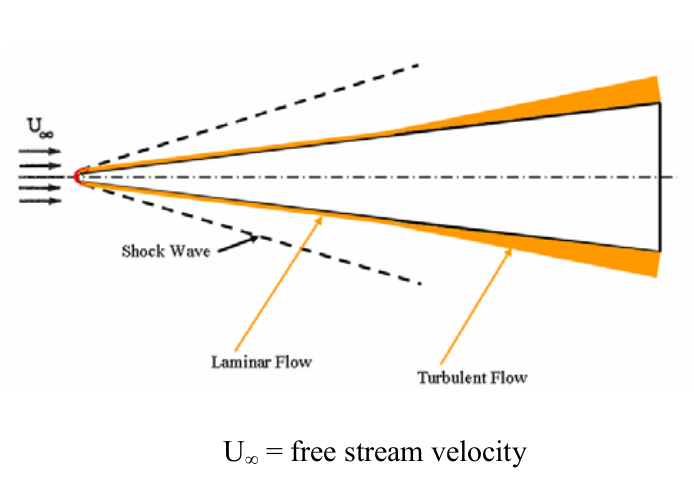
\includegraphics[width=0.8\textwidth]{Images/SlenderBody.png}
		\caption{\textbf{A slender reentry vehicle with an oblique bow shock.}}
		\label{subfig:SlenderBody}
	\end{subfigure}%
	\caption{\textbf{Bow shocks of blunt and slender vehicle geometries. Figures 1 and 2 of \cite{hartunian_implications_2007}}}
	\label{fig:BluntVsSlender}
\end{figure*}

\begin{figure}
	\centering
	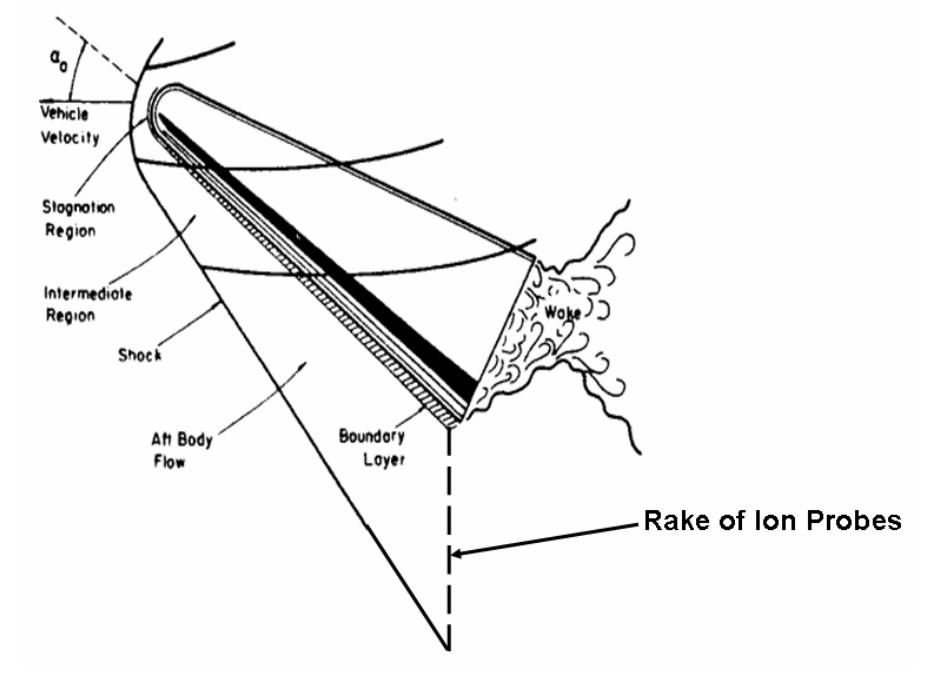
\includegraphics[width=0.5\textwidth]{Images/RAMC_FlowField.png}
	\caption{\textbf{Flow-field diagram of the RAM-C research vehicle.\cite{rybak_causes_1970}\copyright IEEE}}
	\label{fig:RAMCFlowField}
\end{figure}

It was shown analytically in 1958 that a blunt spacecraft design approaching that of a sphere is more desirable over a narrow, streamlined design to minimize heat transfer to the spacecraft.\cite{allen_study_1958}
The ``blunt body" reentry vehicle creates a boundary layer of shock-heated gas in front of it which transfers most heat into the atmospheric gases in the hypersonic flow-field rather than the vehicle itself.
Figure \ref{fig:BluntVsSlender} compare the hypersonic flow-fields of different vehicle shapes.
Figure \ref{fig:RAMCFlowField} shows the anatomy of the flow-field of a blunt reentry vehicle at a non-zero angle of attack.

While a blunt design solves the aerothermodynamic heating problem, the wide bow shock of a blunt body generates a large volume of plasma which infills the volume between the bow shock and the surface of the vehicle.
This results in a dense, thick plasma surrounding the vehicle, increasing the probability of sustained radio blackout.
Slender bodies, on the other hand, produce oblique bow shocks which remain closer to the vehicle's surface, producing a thinner, less dense plasma sheath that is less likely to block radio signals.\cite{hartunian_implications_2007}

Although a slender vehicle design is desirable from a radio communications standpoint, the aerothermodynamic benefits of the blunt body design are far more important for high hypersonic flight and orbital reentry.
As such, we will focus on solutions for the most part which assume a plasma flow field of a blunt body vehicle.


\subsection*{Properties of Hypersonic Plasma Sheaths}
Plasma is a state of matter which is characterized by free-flowing negatively-charged electrons, positive ions, and other neutral atoms and particles.
The free electrons and ions give plasma unique electromagnetic properties not seen in the other states of matter.

An important characteristic property of a plasma is its plasma frequency $\omega_p$ given in units of radians/second by the equation
\begin{equation} \label{plasma_f}
\omega_p = \sqrt{\frac{n_e e^2}{\epsilon_0 m_e}}
\end{equation}
where $e$ is the charge of the electron, $\epsilon_0$ is the permitivity of free space, and $m_e$ is the mass of the electron. 
The quantity $n_e$ is the density of electrons in the plasma.\cite{chen_introduction_1984,kim_analysis_2008}
Equation (\ref{plasma_f}) is interchangeably referred to as the plasma frequency and plasma electron frequency. The plasma frequency given is the resonance frequency of the free electrons about positive ions in the plasma when disturbed by an electromagnetic force such as a radio wave.\cite{chen_introduction_1984}

Since all factors except $n_e$ on the right hand side of  Equation (\ref{plasma_f}) are constants, Equation (\ref{plasma_f}) can be simplified and approximated to
\begin{equation} \label{plasmafapprox}
\omega_p \approx 18\pi\sqrt{n_e}
\end{equation}
As we can see from Equation \ref{plasmafapprox}, the plasma frequency is only dependent on the density of electrons in the plasma, which will hereafter be referred to as the plasma density.

As will be shown in section \ref{sec:Waves}, the plasma frequency is fundamentally important to the radio blackout problem because it is the transmission cutoff frequency for radio waves propagating through a plasma sheath.
A radio wave with carrier frequency $\omega$ that is greater than the plasma frequency $\omega_p$ will propagate through the sheath and reach the vehicle with minor attenuation if any at all, and vice versa from the vehicle to an outside receiver.
Radio waves with frequencies less than or equal to the plasma frequency, on the other hand, will be totally attenuated by and reflected off the plasma sheath, preventing any signals from reaching or leaving the vehicle enveloped in the sheath.

The electron density of a plasma sheath is notoriously difficult to predict and not uniform over the entire sheath.
The plasma density is roughly proportional to the vehicle's velocity and the local atmospheric density.
Because of this, a reentering spacecraft will experience a large range of plasma densities over the duration of its reentry.
The plasma sheath density is also highly dependent on the geometry of the vehicle itself, as was shown in the previous section.

While analytical prediction of plasma densities can be difficult, actual spacecraft atmospheric reentries have given us useful observational data of typical plasma densities and blackout windows for different radio frequencies over varying velocity and altitude.

\begin{figure}[!ht]
	\centering
	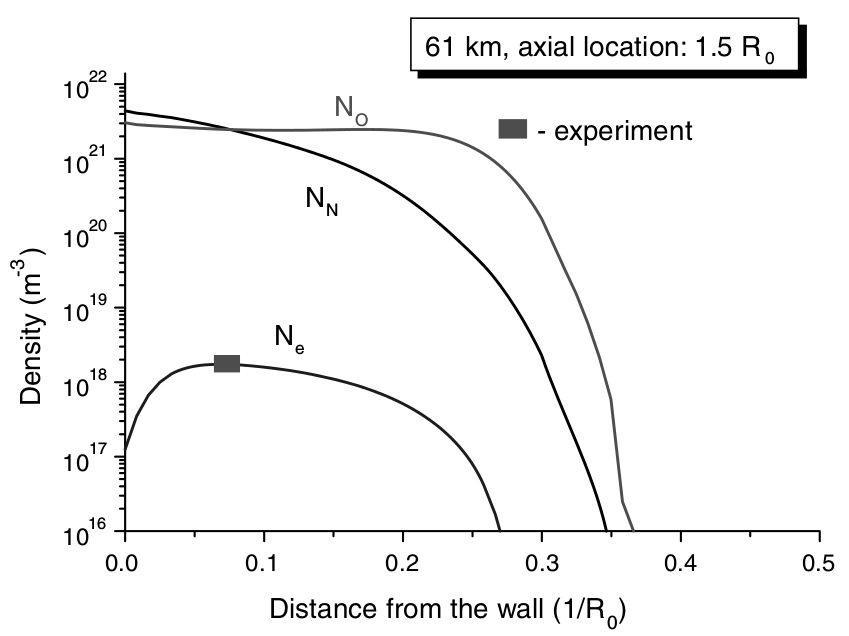
\includegraphics[width=0.5\textwidth]{Images/PlasmaDensity_Keideretal}
	\caption[Computational model of plasma density at varying distances from the vehicle surface.]{\textbf{A computational model of the density of electrons and molecular Oxygen and Nitrogen in the plasma flow-field at varying distances from the vehicle surface. The electron density is compared with experimental density data from project RAM. Figure 2 from \cite{keidar_electromagnetic_2008}}}
	\label{fig:PlasmaDensity_Keideretal}
\end{figure}

Measurements taken during a flight of NASA's RAM program measured typical plasma densities of a vehicle reentering at 7.6 km/s (25,000 ft/s) range from $10^{16}$ to $10^{17}$ electrons per cubic meter between altitudes of 80 and 70 km.\cite{akey_radio_1970}
This corresponds to cutoff plasma frequencies of 900 MHz to 2,850 MHz.

Data taken during the reentry of Mercury 6 at 7.3 km/s (24,000 ft/s) found the peak frequency of the plasma sheath around the location of the antennas to be about 500 GHz, which corresponds to a peak plasma density of $2.11*10^{21} \  m^{-3}$.
The VHF radio blackout duration for Mercury 6 lasted approximately 4.5 minutes from 90 km to 40 km in altitude.
In the stagnation region of the hypersonic flow field, the plasma frequency was found to peak at 6,000 GHz, corresponding to a plasma density of $5*10^{23} m^{-3}$. \cite{lehnert_plasma_1964}

The thickness of the plasma sheath boundary layer was measured during the RAM program using a ``rake" of Langmuir probes which extended into the plasma flow-field up to $0.14m$.\cite{rybak_causes_1970}
Computational modeling of the density profile of the reentry plasma sheath extending from the vehicle surface was done by Keidar et. al. in \cite{keidar_electromagnetic_2008} and verified using project RAM data.
Figure \ref{fig:PlasmaDensity_Keideretal} shows the modeled electron number density $N_e$ peaks near the surface of the vehicle and trails off as distance from the surface increases.

\section{Physics of Waves in Plasma} \label{sec:Waves}
The theory of how electromagnetic waves propagate through and interact with a plasma is important to understanding potential solutions of the radio blackout problem.
What follows is an overview of the physics of electromagnetic and Langmuir waves in plasmas.
For a more detailed and comprehensive introduction to the topic, see chapter 4 of \cite{chen_introduction_1984}, chapter 6 of \cite{papas_theory_1965}, and chapter 9 of \cite{fitzpatrick_maxwells_2008}.

\subsection*{Electromagnetic Waves in a Vacuum}
Before looking at how a plasma effects the propagation of an electromagnetic wave, we first look at how a wave travels in a vacuum.
We start with a brief overview of Maxwell's equations:

\begin{equation}
	\label{eq:MaxVacGaussE}
	\nabla \cdot \mathbf{E} = 0
\end{equation}
\begin{equation}
	\nabla \cdot \mathbf{B} = 0
\end{equation}
\begin{equation} 
	\label{eq:MaxVacCurlE}
	\nabla \times \mathbf{E} = -\frac{1}{c} \frac{\partial \mathbf{B}}{\partial t}
\end{equation}
\begin{equation} 
	\label{eq:MaxVacCurlB}
	\nabla \times \mathbf{B} = \frac{1}{c^2} \frac{\partial \mathbf{E}}{\partial t}
\end{equation}

If we take the curl of equation (\ref{eq:MaxVacCurlE}) and the partial time derivative of equation (\ref{eq:MaxVacCurlB}), we have

\begin{equation}
	\label{eq:CurlVacCurlE}
	\nabla \times ( \nabla \times \mathbf{E}) = \nabla \times (-\frac{1}{c} \frac{\partial \mathbf{B}}{\partial t}) 
\end{equation}
\begin{center}
	and
\end{center}
\begin{equation}
	\label{eq:PartialVacCurlB}
	\nabla \times \frac{\partial \mathbf{B}}{\partial t} = \frac{1}{c} \frac{\partial^2 \mathbf{E}}{\partial t^2}
\end{equation}
Substituting (\ref{eq:PartialVacCurlB}) into (\ref{eq:CurlVacCurlE}),
\begin{equation}
	\nabla \times ( \nabla \times \mathbf{E}) = -\frac{1}{c^2} \frac{\partial^2 \mathbf{E}}{\partial t^2} 
\end{equation}
Using the vector identity
\begin{equation}
	\label{eq:NablaIdent}
	\nabla \times (\nabla \times \mathbf{E}) = \nabla(\nabla \cdot \mathbf{E}) - \nabla^2\mathbf{E}
\end{equation}
And the Maxwell Equation $\nabla \cdot \mathbf{E} = 0$, we have:
\begin{equation}
	\label{eq:VacWaveEqtn}
	\nabla^2\mathbf{E} - \frac{1}{c^2} \frac{\partial^2 \mathbf{E}}{\partial t^2} = 0
\end{equation}
Equation (\ref{eq:VacWaveEqtn}) is the wave equation for the electric field in a vacuum, with
\begin{equation}
	c^2 = \frac{1}{\epsilon_0 \mu_0}
\end{equation}

The plane wave solutions of this equation take the form $\mathbf{E}(\mathbf{r}, t) = e^{i(\mathbf{k} \cdot \mathbf{r} - \omega t)}$, where $\mathbf{k}$ is the wave vector which points in the direction of the phase velocity, and $\mathbf{r}$ is the position vector.
When the plane wave solution is substituted into (\ref{eq:VacWaveEqtn}), we arrive at
\begin{equation}
	k^2\mathbf{E} - \frac{\omega^2}{c^2}\mathbf{E} = 0
\end{equation}
Which reduces to the dispersion relation of the wave given by
\begin{equation}
	\omega^2 = k^2c^2
\end{equation}

The quantity $c$ is the phase velocity $\frac{\omega}{k}$ of the light waves which in a vacuum is, of course, the speed of light in a vacuum given by $c = \frac{1}{\sqrt{\mu_0\epsilon_0}}$.

\subsection*{Electromagnetic Waves in a Plasma}
Our goal now is to find the dispersion relation of an electromagnetic wave traveling through an unmagnetized plasma.
Since the wave now propagates through a plasma, we must include the extra term $\mathbf{j}/\epsilon_0$ in equation (\ref{eq:MaxVacCurlE}) to account for the currents of charged particle motions.
Our relevant Maxwell's equations (\ref{eq:MaxVacCurlE}) and (\ref{eq:MaxVacCurlB}) then become:
\begin{equation}
	\label{eq:MaxPlasCurlE}
	\nabla \times \mathbf{E} = -\frac{1}{c} \frac{\partial \mathbf{B}}{\partial t}
\end{equation}
\begin{equation}
	\label{eq:MaxPlasCurlB}
	\nabla \times \mathbf{B} = \frac{1}{c} (\frac{\partial \mathbf{E}}{\partial t} + \frac{\mathbf{j}}{\epsilon_0})
\end{equation}

Once again taking the curl of (\ref{eq:MaxPlasCurlE}) and applying the vector identity in (\ref{eq:NablaIdent}):
\begin{equation}
	\label{eq:PlasCurlCurlE}
	\nabla \times (\nabla \times \mathbf{E}) = \nabla(\nabla \cdot \mathbf{E}) - \nabla^2 \mathbf{E} = -\frac{1}{c}\nabla \times \frac{\partial \mathbf{B}}{\partial t}
\end{equation}

And taking the time derivative of (\ref{eq:MaxPlasCurlB}):
\begin{equation}
	\label{eq:PlasCurlPartialB}
	\nabla \times \frac{\partial \mathbf{B}}{\partial t} = \frac{1}{c}(\frac{\partial^2 \mathbf{E}}{\partial t^2} + \frac{1}{\epsilon_0} \frac{\partial \mathbf{j}}{\partial t})
\end{equation}

We finally substitute (\ref{eq:PlasCurlPartialB}) into (\ref{eq:PlasCurlCurlE}) and arrive at the wave equation

\begin{equation}
	\nabla^2 \mathbf{E} = \frac{1}{c^2}(\frac{\partial^2 \mathbf{E}}{\partial t^2} + \frac{1}{\epsilon_0} \frac{\partial \mathbf{j}}{\partial t})
\end{equation}

Substituting the plane wave solution $\mathbf{E} = e^{i(\mathbf{k} \cdot \mathbf{r} - \omega t)}$:
\begin{equation}
	\label{eq:PlasPlaneWave1}
	k^2\mathbf{E} = \frac{\omega^2}{c^2}\mathbf{E} + \frac{i\omega}{\epsilon_0 c^2}\mathbf{j}
\end{equation}
In this case, we are considering radio and microwave radiation with frequencies on the order of $10^6$ to $10^9$.
Because the radiation frequency is high, the ions in the plasma can be considered fixed in space, and the current $\mathbf{j}$ comes entirely from electron motion:
 
\begin{equation}
	\mathbf{j} = -n_ee\mathbf{v_e}
\end{equation}
Where $n_e$ is the electron number density, $e$ is the charge of the electron, and $\mathbf{v_e}$ is the average electron velocity in the plasma.

From the linearized electron equation of motion with negligible thermal motion such that $KT_e = 0$, we have
\begin{equation}
	m_e\frac{\partial \mathbf{v_e}}{\partial t} = -e\mathbf{E}
\end{equation}
\begin{equation}
	\mathbf{v_e} = \frac{e\mathbf{E}}{im_e\omega}
\end{equation}
Thus the electron current $\mathbf{j}$ is given by:
\begin{equation}
	\mathbf{j} = -n_ee^2\frac{\mathbf{E}}{im_e\omega}
\end{equation}
Substituting this back into the plane wave equation (\ref{eq:PlasPlaneWave1})
\begin{equation}
	k^2\mathbf{E} = \frac{\omega^2}{c^2}\mathbf{E} - \frac{i\omega}{\epsilon_0 c^2}n_ee^2\frac{\mathbf{E}}{im_e\omega}
\end{equation}
Which reduces to:
\begin{equation*}
	c^2k^2 = \omega^2 - \frac{n_ee^2}{\epsilon_0m_e}
\end{equation*}
Comparing this to equation (\ref{plasma_f}), we see that the second term on the right is just the plasma frequency squared, and so we arrive at the dispersion relation
\begin{equation}
	\omega^2 = \omega^2_p + c^2k^2
\end{equation}

The wavenumber for an electromagnetic wave propagating through a plasma is then given by:
\begin{equation}
	\label{eq:EMWaveNumber}
	k = \frac{1}{c}\sqrt{1-\frac{\omega^2_p}{\omega^2}}	
\end{equation}
Where $\omega_p$ is the plasma frequency, and $\omega$ is the frequency of the electromagnetic wave.
In multi-dimensional space, the wavenumber is a vector which points in the direction of the wave's propagation.

Examining equation \ref{eq:EMWaveNumber}, we can see that there are three special cases of $k$ that are dependent on the ratio $\omega_p/\omega$:
\begin{description}
	\item [Case 1]$\omega > \omega_p \Rightarrow$ k is real.
	\item [Case 2]$\omega < \omega_p \Rightarrow$ k is imaginary.
	\item [Case 3]$\omega = \omega_p \Rightarrow$ k is zero.
\end{description}

In case one where the frequency of the wave is greater than the plasma frequency, the wave will propagate through the plasma (one-dimensionally in the $x$-direction) according to the wave equation $E(x,t) = Ae^{i(kx - \omega t)}$.

In case two, the wave frequency is less than the plasma frequency, which results in an imaginary wavenumber $k = i\gamma$.
Substituting this into the wave equation:
\begin{equation}
	E(x,t) = e^{i(i\gamma)x - i\omega t} = e^{-\gamma x}e^{i\omega t}
\end{equation}
Thus, the effect on the electromagnetic wave is that it is exponentially damped according to $e^{-\gamma x}$ as it travels through the plasma.

In the third case, where the wave frequency equals the plasma frequency, the wavenumber is exactly zero, and the wave is reflected by the plasma.

To illustrate the importance of this, imagine a radio wave emitted by a ground station traveling to a reentering spacecraft.
As the radio wave comes into contact with the plasma flow-field, the outer portion of the plasma sheath will be less dense, and therefore have a lower frequency than the radio wave, and so the wave propagates through the plasma initially.
As the wave travels further into the plasma sheath, the plasma becomes denser, and its frequency increases until the plasma frequency equals the radio wave's frequency.
At this point, further travel into the plasma sheath will be damped exponentially, and the radio wave will be reflected.
This is the primary mechanism by which the radio blackout occurs.

\subsection*{Plasma Oscillations}
We now turn our attention to oscillations of the charged particles of the plasma itself.
One of our fundamental assumptions will be that positive ions in the plasma are fixed, and all subsequent oscillatory motion will exclusively be that of electrons in the plasma.
While this is not strictly accurate, it is an adequate assumption because we are primarily considering radio-frequency electromagnetic waves on the order of $10^6$ to $10^9$ Hertz.

We start with the general electron fluid equation of motion in the presence of an electric field given by
\begin{equation} \label{eq:emotionhot}
m_en_e \lbrack \frac{\partial \mathbf{v_e}}{\partial t} + \left( \mathbf{v_e} \cdot \mathbf{\nabla} \right) \mathbf{v_e} \rbrack = -en_e\mathbf{E} - \nabla p
\end{equation}
Where $m_e$ is the mass of the electron, $n_e$ is the electron number density, $\mathbf{v_e}$ is the average electron velocity, $e$ is the electron charge, $\mathbf{E}$ is the electric field acting on the electron, and $p$ is the thermal motion pressure.

We can derive two very different behaviors of the plasma from Equation (\ref{eq:emotionhot}) depending on whether we retain the pressure gradient term $\nabla p$.

If we leave out the thermal motion of the electrons and, therefore, the pressure gradient term, we can derive a wave equation for the electrons with a frequency given by the plasma frequency in Equation (\ref{plasma_f}).
Furthermore, these plasma oscillations do not propagate forward into the plasma and remain local to individual electron-ion pairs.

If thermal motion is considered, the pressure gradient term of the electron fluid must be included in the equation of motion of the electrons, and the resulting wave equation shows that the oscillation does in fact propagate through the plasma as a plasma wave, or a Langmuir wave.

In this section, we will consider the first case, where thermal motion is ignored and the plasma oscillations remain stationary.
In the next section, we will consider the latter case where thermal motion is included and plasma disturbances do propagate as Langmuir waves.

Although electron thermal motion is significant in real plasmas, both cases are important to consider since they describe how plasma interacts with electromagnetic waves.

When electrons in a homogeneous non-ionized plasma are displaced, Coulomb forces between electrons and positive ions build up electric fields which restore the net-neutrality of the plasma.
The restoring forces return electrons towards equilibrium with respect to the ions, but the inertia of the electrons cause them to overshoot the ions and begin to oscillate.

In the derivation of the plasma frequency, we assume the following:
\begin{enumerate}
	\item The plasma is not magnetized.
	\item There are no thermal motions.
	\item The ions are fixed in space in a uniform distribution due to their greater inertia.
	\item The plasma is infinite in extent.
	\item The electron motions are one dimensional in the $x$ direction.
\end{enumerate}

The electron equation of motion resulting from the restoring Coulomb forces is given by
\begin{equation} \label{eq:emotion}
	m_en_e \lbrack \frac{\partial \mathbf{v_e}}{\partial t} + \left( \mathbf{v_e} \cdot \mathbf{\nabla} \right) \mathbf{v_e} \rbrack = -en_e\mathbf{E}
\end{equation}
The right-hand side of equation (\ref{eq:emotion}) represents the restoring force of the unbalanced electric fields, and the first term on the left-hand side is a simple $m\cdot\mathbf{a}$ expression.
The second term on the left encapsulates the bulk fluid motion of the electrons in the plasma field.

We will also need the electron equation of continuity:
\begin{equation}
	\frac{\partial n_e}{\partial t} + \mathbf{\nabla} \cdot (n_e \mathbf{v_e}) = 0
	\label{eq:ElectronContinuity}
\end{equation}

If we linearize Equation (\ref{eq:emotion}) and assume the oscillation of the electrons is small, the term $\left(\mathbf{v_e} \cdot \nabla \right) \mathbf{v_e}$ can be ignored.
The equation of motion then reduces to:
\begin{equation}
	m \frac{\partial \mathbf{v_e}}{\partial t} = -e \mathbf{E}
	\label{eq:EmotionLinear}
\end{equation}

Since we are now looking at waves in a plasma, our Maxwell equations must be slightly altered to account for charge densities and currents.
Equation \ref{eq:MaxVacGaussE}, Gauss's Law, becomes:
\begin{equation}
	\label{eq:MaxGaussE}
	\mathbf{\nabla} \cdot \mathbf{E} = \frac{\rho}{\epsilon_0}
\end{equation}
And Equation (\ref{eq:MaxVacCurlB}), Amp\'{e}re's Law, becomes:
\begin{equation}
	\label{eq:MaxCurlB}
	\mathbf{\nabla \times B} = \mu_0 \left( \mathbf{J} + \epsilon_0 \frac{\partial \mathbf{E}}{\partial t} \right)
\end{equation}

Gauss's Law in one dimension is used to find the $\mathbf{E}$ based on the relative charge density difference between ions and electrons.
\begin{equation} 
	\epsilon_0 \mathbf{\nabla \cdot E} = \epsilon_0 \frac{\partial\mathbf{E}}{\partial x} = e(n_i - n_e)
	\label{eq:Poisson}
\end{equation}

Equation (\ref{eq:Poisson}) can be solved by the process of linearization in which the oscillations of the electrons are broken into the equilibrium state and the ``perturbed" state.
In the equilibrium state, $n_i = n_e$.
By the assumption of fixed ions, however, $n_i = 0$ in the perturbed state.
Thus, in the perturbed state, Equation (\ref{eq:Poisson}) becomes:
\begin{equation}
	\epsilon_0\mathbf{\nabla \cdot E} = -en_e
	\label{eq:PoissonSimple}
\end{equation}

Modeling the electron velocity, the restoring electric field, and the density of perturbed electrons sinusoidally:
\begin{equation*}
	v_x = v_xe^{i(kx - \omega t)}
\end{equation*}
\begin{equation*}
	n_e = n_e^{i(kx-\omega t)}
\end{equation*}
\begin{equation*}
	E = Ee^{i(kx-\omega t)}
\end{equation*}

We replace the time derivatives $\partial/\partial t$ with $-i\omega$ and the spatial derivatives $\mathbf{\nabla}$ with $ikx$.
Equations (\ref{eq:ElectronContinuity}) (\ref{eq:EmotionLinear}), (\ref{eq:PoissonSimple}), and  then become:
\begin{equation*}
	-i\omega n_e = -ikn_ev_e
\end{equation*}
\begin{equation*}
	-i\omega m_E v_e= -eE
\end{equation*}
\begin{equation*}
	ik\epsilon_0E = -en_e
\end{equation*}

When we solve this system of equations for $\omega$, we arrive at:
\begin{equation}
	\omega^2 = \frac{e^2 n_e}{m_e\epsilon_0}
\end{equation}
Which is identical to the plasma frequency given by equation (\ref{plasma_f}).

Since the plasma frequency has no dependence on the wave number $k$, the group velocity $v_g = d\omega/dk$ is zero, and the wave does not propagate.
This oscillation is then simply the stationary resonance frequency of the electrons about the fixed ions in the plasma.
\subsection*{Plasma (Langmuir) Waves}
	We now turn our attention to the more accurate case where electron thermal motion is included.
	In this case, we return to using Equation \ref{eq:emotionhot} to describe the motion of electrons in the plasma, this time including the pressure gradient term.
	The thermal velocities of the electrons will cause longitudinal movement, thus carrying information of the disturbance oscillations throughout the plasma.
	
	We proceed with similar steps as the previous section, but this time we include the pressure gradient term $\nabla p = 4kT_e\nabla n_e$.
	The resulting dispersion relation of the electron oscillations is given by:
	
	\begin{equation*}
		\omega^2 = \frac{n_e e^2}{\epsilon_0 m_e} + \frac{3kT_e}{m}k^2
	\end{equation*}
	\begin{equation}
		\omega^2 = \omega^2_p + \frac{3}{2}k^2 v_{th}
	\end{equation}
	Where $v_th \equiv 2kT_e/m_e$ is the thermal velocity of the electrons.
	This oscillation now depends on $k$, so the group velocity is non-zero, and thus propagates through the plasma with speed:
	\begin{equation}
		v_g = \frac{d\omega}{dk} = \frac{3k}{2\omega}v^2_{th}
	\end{equation}
	
	These propagating oscillations in plasmas are also known as Langmuir waves, and present a potential solution to communicating through plasma sheaths by inducing Langmuir waves which can carry information through the plasma.
	



\section{Overview of Solutions} \label{sec:Overview}
	We will now look at several potential solutions to the radio blackout problem which have been previously studied.
	All potential solutions generally break down into two categories: passive techniques and active techniques.
	
	\subsection*{Passive Techniques}
		Passive techniques involve designing the vehicle or mission profile to minimize or eliminate radio blackout.
		This includes altering the shape of the vehicle to produce thinner and less dense plasma sheaths, a technique known as aerodynamic shaping.
		Selecting a flight profile or reentry trajectory which minimizes aerodynamic heating and plasma generation is also a passive solution.
		
		The primary detraction of passive solutions, however, is that they rely on designing the vehicle around the minimization of the plasma sheath and the radio blackout.
		Depending on the mission requirements of a vehicle, this could make passive solutions undesirable to implement because of their affect on the vehicle's mass or aerodynamic properties.
		
		\subsubsection{Aerodynamic Shaping}
			In section \ref{sec:PlasmaSheaths}, it was shown that the shape of the vehicle dramatically effects the properties of the plasma sheath, and that streamlined, slender shapes create oblique shock waves which produce less plasma than the wide bow shock of a blunt body.
			Despite this, blunt bodies have more favorable aerothermodynamic properties for reentry vehicles, and so blunt body designs dominate spacecraft reentry capsules.
			
			To minimize the radio blackout conditions of a blunt body vehicle, alternate means of shaping the plasma sheath have been studied.
			``Spike" structures which protrude into the stagnation region of the plasma flow-field can be used to create a more oblique shock wave which produces less plasma around the separated flow regions aft of the vehicle where antennas might be located.\cite{hartunian_implications_2007}
			Spike structures could also be used to place an antenna outside of the plasma sheath altogether.\cite{belov_investigation_2001}
			 
			The major issue with aerodynamic shaping structures is, once again, the aerodynamic heating problem.
			The spike structure must be insulated somehow from the hottest part of the plasma flow-field, otherwise it will be destroyed relatively quickly.\cite{hartunian_implications_2007}
			Active cooling systems could be used to protect the spike structure, but this begins to add weight and complexity.
			
	\subsection*{Active Techniques}
		Active methods of solving the radio blackout problem involve active systems which either affect the properties of the plasma sheath to allow radio waves to pass through, or exploit other mechanisms to communicate across the plasma barrier.
		In this section, we'll summarize the most prominent active techniques.
	
		\subsubsection*{High-Frequency Radio}
			Perhaps the simplest solution to the radio blackout problem is the most obvious: use radio waves with frequencies higher than the plasma frequency to communicate.
			As was shown in section \ref{sec:Waves}, electromagnetic waves with frequency higher than the plasma frequency will not be attenuated.
			In section \ref{sec:PlasmaSheaths} it was shown that typical orbital reentry peak plasma frequencies range from 3GHz to 500 GHz.
			
			Table \ref{tab:RadioBands} shows the common radio band designations and frequency ranges.
			VHF and UHF are most commonly used for aircraft and spacecraft voice and data telemetry, but have relatively low frequencies, making them more susceptible to being attenuated by a plasma sheath.
			Above VHF and UHF are the microwave bands which are commonly used for spacecraft data transmission and telemetry.
			As Table \ref{tab:RadioBands} shows, higher frequency bands such as the K band could be used to overcome the radio blackout for hypersonic atmospheric cruise, and reduce or totally remove the duration of low earth orbit reentry blackouts.
			
			% ieee radio bands
			\begin{table}[h]	
				\centering
				\begin{tabular}{c|c}
					Band    & Frequency range   \\ \hline
					HF      & 0.003 - 0.03 GHz \\
					VHF     & 0.03 - 0.3 GHz   \\
					UHF     & 0.3 - 1 GHz      \\
					L       & 1 - 2 GHz        \\
					S       & 2 - 4 GHz        \\
					C       & 4 - 8 GHz        \\
					X       & 8 - 12 GHz       \\
					Ku      & 12 - 18 GHz      \\
					K       & 18 - 27 GHz      \\
					Ka      & 27 - 40 GHz      \\
					V       & 40 - 75 GHz      \\
					W       & 75 - 110 GHz     \\
					mm or G & 110 - 300 GHz​  
				\end{tabular}
				\caption{\textbf{IEEE radio frequency bands.}}
				\label{tab:RadioBands}
			\end{table}
			
			The primary problem with using high-frequency radiation for vehicle-to-ground communication is the attenuation by atmospheric water vapor and gases such as molecular Oxygen.
			As Figure \ref{fig:RadioAttenuation} shows, the atmospheric attenuation penalty increases rapidly as the wavelength of the radio wave decreases.
			For frequencies above approximately 10 GHz, atmospheric attenuation becomes a significant even in dry atmospheric conditions, making the effectiveness of using high-frequency microwaves to solve the radio blackout problem limited.\cite{hartunian_implications_2007}
		
			% atmospheric radio attenuation plot.
			\begin{figure}[H]
				\centering
				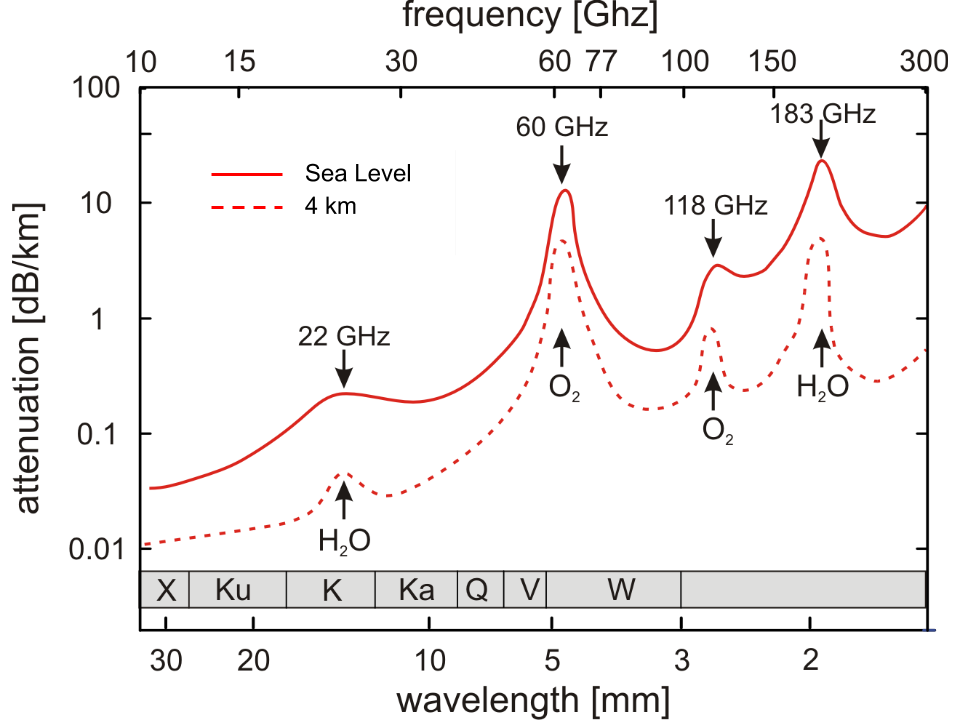
\includegraphics[width=0.45\textwidth]{Images/intro-atmospheric.png}
			\caption{\textbf{Atmospheric attenuation of radio waves by wavelength. Radio bandwidths are shown along the bottom horizontal axis.\cite{altshuler_comparison_1988} \copyright IEEE 1988.}}
			\label{fig:RadioAttenuation}
			\end{figure}
		
			Beyond the microwave band of electromagnetic radiation, the atmosphere becomes transparent again to light waves, posing another possible solution.
			Research into Earth-to-space high-bandwidth optical communication has been conducted by the NASA Jet Propulsion Lab since 2014.
			The Optical Payload for Lasercomm Science (OPALS) is an experimental optical communications system currently on-board the International Space Station that is being used to study the feasibility of such communications.
			The OPALS system uses a 1,550nm 2.5W laser to communicate with a ground station on Earth, downlinking video data at 50Mb/s.\cite{oaida_optical_2014}
			Initial results have been promising, however there is a strict requirement on pointing accuracy of the laser, unlike radio and microwave signals. \cite{abrahamson_achieving_2015}
		
		\subsubsection*{Liquid Quenching}
			A technique that has been studied and even flight tested with success is injecting a liquid such as water into the plasma flow field.
			The primary mechanism at work is the recombination of electrons and ions at or near the surface of water drops, thereby artificially reducing the electron number density in the plasma.\cite{evans_reduction_1965}
			
			Liquid quenching was first tested by NASA on the RAM B-2 and C-1 flights in the mid 1960's. \cite{rybak_causes_1970}
			Both flights used water as a quenching substance.
			Initial results were mixed, though RAM C-1 did measure a decrease in the plasma density during injection.
			Figure \ref{fig:RAMCWaterInject} shows the plasma density around the RAM C-1 vehicle during a series of water injection tests of varying flow rates.
			
			
			\begin{figure}
				\centering
				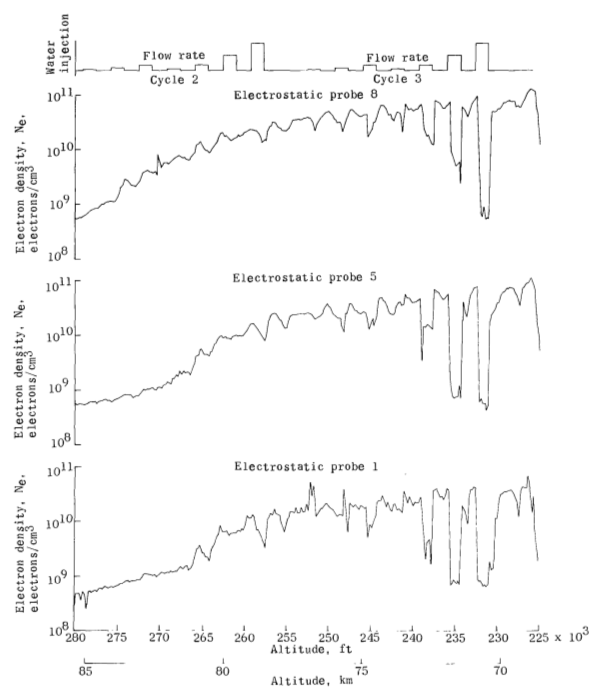
\includegraphics[width = 0.5\textwidth]{Images/RAMC_LangmuirWaterFlow.png}
				\caption{\textbf{Electron number density measurements over altitude from three electrostatic probes located 1, 4.5, and 7cm from the surface of the RAM C-1 vehicle during the water injection experiment. Figure 19 of \cite{akey_radio_1970}}}
				\label{fig:RAMCWaterInject}
			\end{figure}
			
			Liquid quenching was again tested on RAM C-C, this time using alternate injections of perfluoro-octane and water.\cite{rybak_causes_1970}
			
			The last time liquid quenching was tested in flight was during Gemini 3, the first crewed Gemini mission.\cite{schroeder_flight_1968}
			During reentry, an astronaut manually operated the experiment, which injected water at varying flow rates into the plasma flow-field.
			Figure \ref{fig:GeminiWaterDiagram} depicts the configuration of the Gemini water injection experiment.
			The results of the Gemini experiment were much more promising, and significant increases in signal strength during the radio blackout period of both VHF and C-band radio was observed during water injection periods.\cite{schroeder_flight_1968}
			\begin{figure}
				\centering
				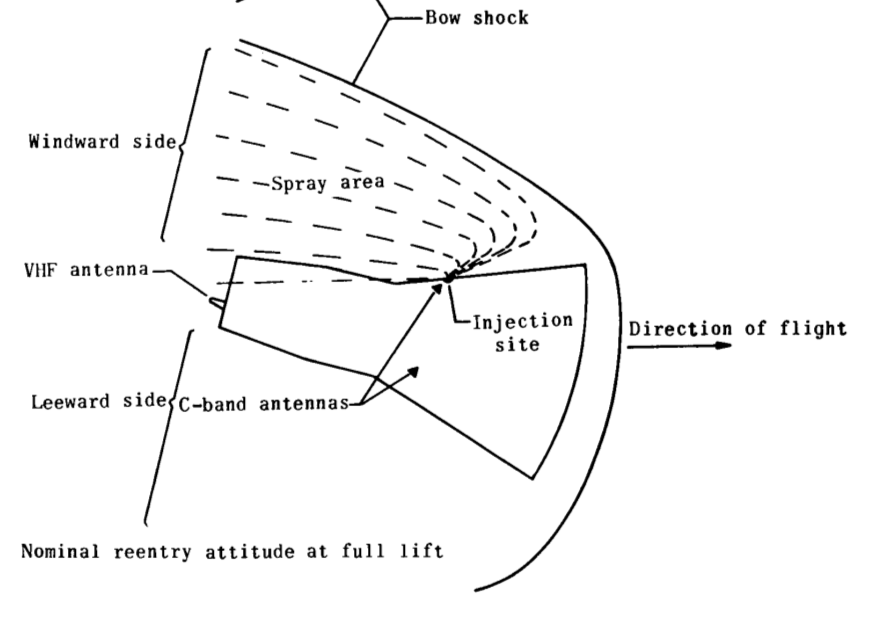
\includegraphics[width=0.4\textwidth]{Images/GeminiWaterDiagram}
				\caption[Diagram of the Gemini 3 water injection experiment.]{\textbf{The Gemini 3 water injection experiment. The spray area was designed to reduce plasma temperature and density over the C-band and VHF antennas. Figure 2 of \cite{schroeder_flight_1968}.}}
				\label{fig:GeminiWaterDiagram}
			\end{figure}
			
			The primary disadvantage of the water injection technique is the engineering complexity of an injection system, as well as mass and volume.
			A pressurization system with associated plumbing an electrical systems is required to achieve adequate penetration of the plasma sheath by the water to create a communication window.
			In order to create a sustained window throughout the entire blackout period, a significant reservoir of water must be carried as well.
			This is mass that must be carried for the entire mission in order to create a communication window for several minutes.
			Depending on the parameters of the mission, this could be a hugely prohibitive cost associated with mitigating the blackout problem.
		
		\subsubsection*{Magnetic Windows}
			Solutions which use static magnetic fields to create windows through which radio-frequency signals could propagate have been studied since the 1960's.\cite{russo_measurements_1964}
			A static magnetic field would theoretically restrain electrons along magnetic field lines, artificially reducing the effective plasma frequency and creating a window through which signals could propagate.\cite{kim_electromagnetic_2009}
			
			Several issues exist with using static magnetic fields as a solution, chief among them being the size and weight of the required electromagnet.
			Past research has found that field strengths on the order of 1 to 2 Tesla would be required to effect significant reduction in the attenuation of signals through the window.\cite{otsu_feasibility_2006}\cite{kim_electromagnetic_2009}
			The requisite electromagnet to produce such a field would exceed 500kg.
			Additional problems arise with the size of the electromagnet required to create a uniform field over a significant area.\cite{kim_electromagnetic_2009}
			
		
		\subsubsection*{Lorentz Windows}
			The Lorentz window method uses crossed electric and magnetic fields to create a local region of relatively low density in the plasma sheath over an antenna on the vehicle, thereby lowering the plasma frequency and creating a window through which radio waves could propagate.
			The method is named so because the primary mechanism is the transport of electrons using the Lorentz force.
			
			Kim et. al. have developed computer numerical simulations of a possible Lorentz window configuration using static crossed electric and magnetic fields on the surface of a vehicle.\cite{kim_plasma_2007}\cite{kim_analysis_2008}\cite{kim_modeling_2010}
			The basic concept involves placing an antenna under perpendicular electric and magnetic fields which reduce the plasma density in the volume directly above the antenna by accelerating ions and electrons out of the volume.
			The configuration proposed by Kim et. al. is shown in Figure \ref{fig:KimExBConfig}.
			Because smaller magnetic fields on the order $0.1 T$ are required to achieve an effect, this method could be more feasible than using static magnetic fields alone.
		
			\begin{figure}[H]
				\centering
					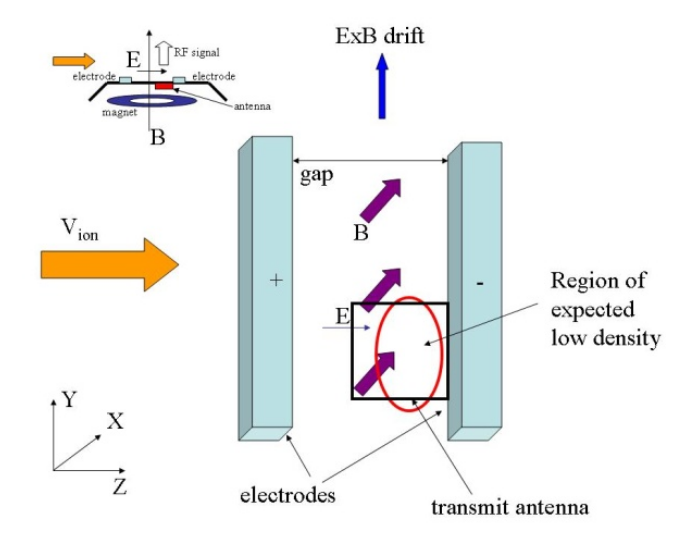
\includegraphics[width=0.45\textwidth]{Images/Kimetal_ExB_config.png}
				\caption{\textbf{Proposed configuration of electrodes and magnetic field for a Lorentz window. Figure 1 in \cite{kim_plasma_2007}.}}
				\label{fig:KimExBConfig}
			\end{figure}
			
			\begin{figure}[!ht]
				\centering
				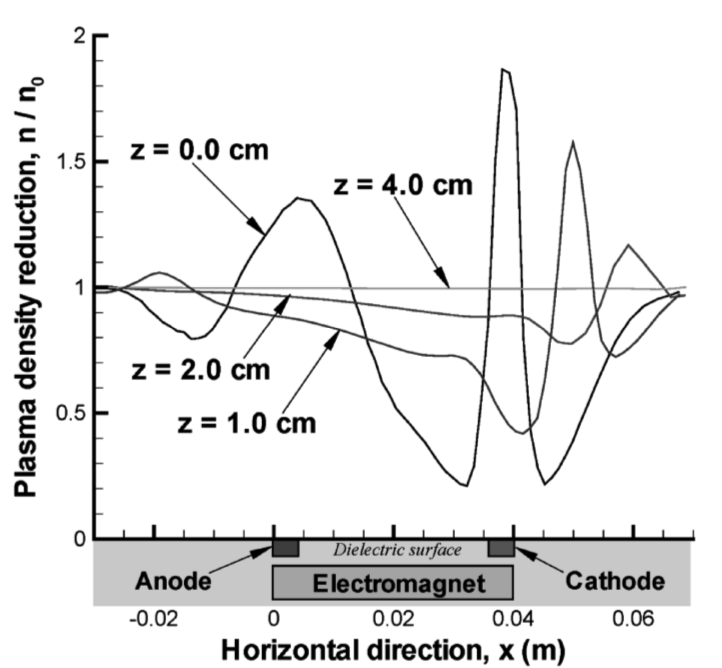
\includegraphics[width=0.5\textwidth]{Images/Kim_DensityReduction}
				\caption[Simulated plasma density reduction of an ExB field.]{\textbf{Plasma density reduction ratios at different distances $z$ from the vehicle surface. Figure 6 of \cite{kim_modeling_2010}}}
				\label{fig:Kim_DensityReduction}
			\end{figure}
			
			\begin{figure}[!ht]
				\centering
				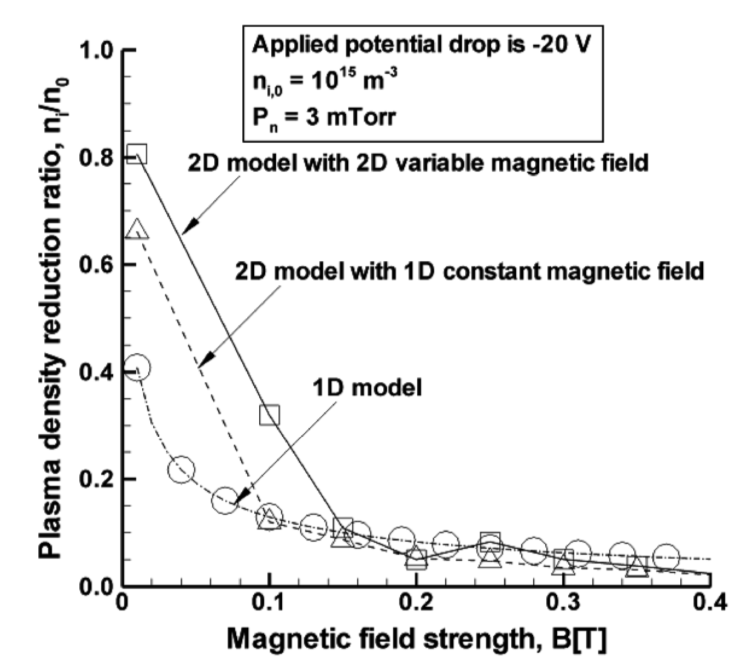
\includegraphics[width=0.5\textwidth]{Images/Kim_DensityModeling}
				\caption[Density reduction ratio of an ExB field with different models.]{\textbf{The plasma density reduction ratios of three different models. More accurate models show less favorable results in plasma reduction. Figure 8 of \cite{kim_modeling_2010}}}
				\label{fig:Kim_DensityModeling}
			\end{figure}
			
			The computer simulations done by Kim et. al. suggest that such an $\mathbf{E \times B}$ configuration could be effective in creating a window of decreased plasma density stretching several centimeters into the boundary layer of the plasma flow-field.
			Figure \ref{fig:Kim_DensityReduction} shows the plasma density reduction ratios of the simulated Lorentz window configuration by Kim et. al..
			These results are promising, because they show the low-density window could extend past the region of highest plasma density in the flow-field.\cite{kim_modeling_2010}
			
			
			
			These studies attempt to model highly complex plasma interactions, however.
			Figure \ref{fig:Kim_DensityModeling} shows that increasingly accurate models of the plasma flow-field and ExB fields have less promising plasma reduction characteristics.
			Important to verifying the viability of Lorentz windows will be additional lab experimentation with real plasmas, as well as real-world flight testing.
			

			
			\begin{figure*}[!ht]
				\centering
				\begin{subfigure}{0.5\textwidth}
					\centering
					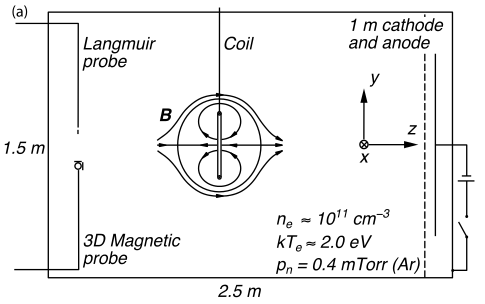
\includegraphics[width=1.0\textwidth]{Images/Stenzel_ExperimentConfig1}
					\label{fig:Stenzel_ExperimentConfig1}
					\caption{\textbf{Overview of the experimental configuration, looking edge-on to the wire loop.}}
				\end{subfigure}%
				\begin{subfigure}{0.5\textwidth}
					\centering
					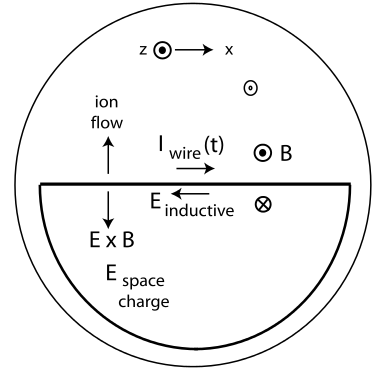
\includegraphics[width=1.0\textwidth]{Images/Stenzel_ExperimentConfig2}
					\caption{\textbf{Detail of the wire loop.}}
					\label{fig:Stenzel_ExperimentConfig2}
				\end{subfigure}%
				\caption{\textbf{Configuration of the pulsed-current $\mathbf{E\times B}$ experiment by Stenzel and Urrutia.}\cite{stenzel_new_2013}}
				\label{fig:Stenzel_ExperimentConfig}
			\end{figure*}
			
				\begin{figure}[!th]
					\centering
					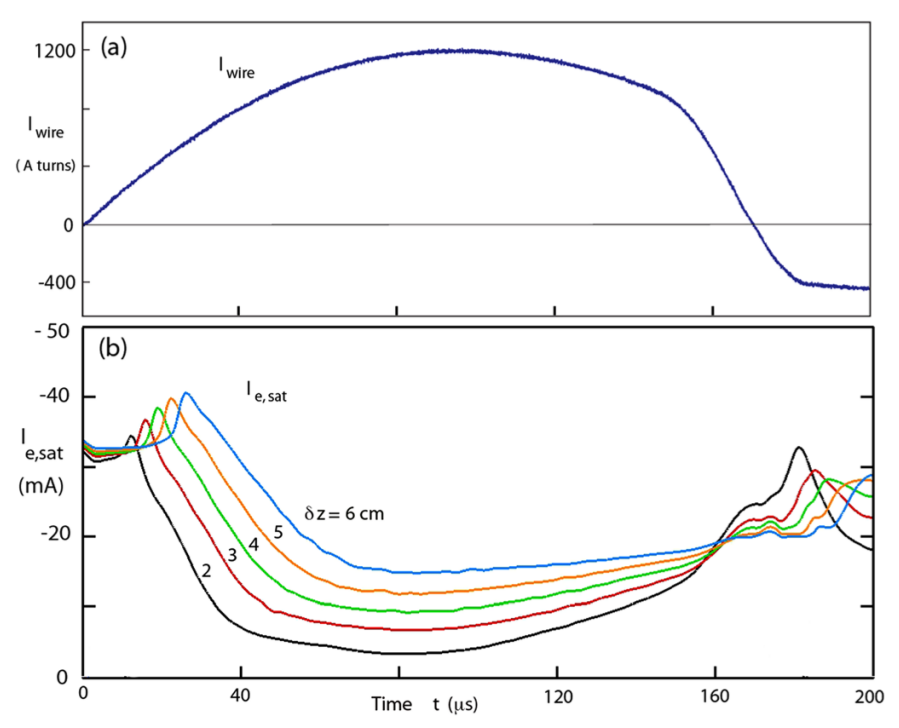
\includegraphics[width=0.5\textwidth]{Images/Stenzel_ExperimentCurrentPlots}
					\caption{\textbf{Plasma density in the vicinity of the wire loop during a rising current pulse. The top figure shows the current through the wire over time. The bottom plot shows the Langmuir probe saturation current at varying distances from the coil during the pulse. Figure 3 of \cite{stenzel_new_2013}}}
					\label{fig:Stenzel_ExperimentCurrentPlots}
				\end{figure}
				
				\begin{figure*}[!ht]
					\centering
					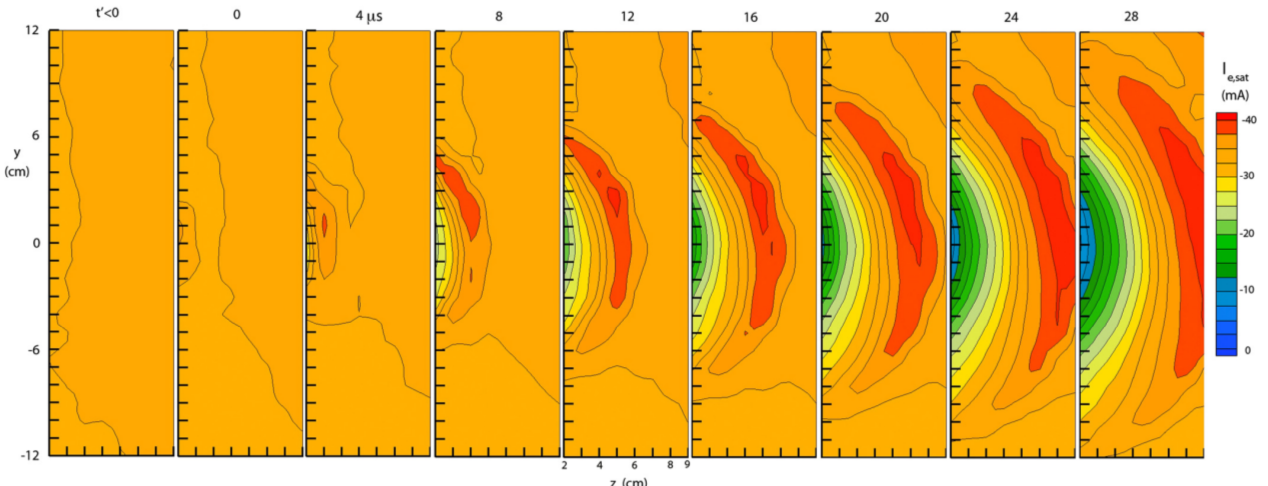
\includegraphics[width=1.0\linewidth]{Images/Stenzel_ExperimentContourPlot}
					\caption{\textbf{Langmuir probe ion saturation during a current pulse. A wave of higher density plasma travels outwards, followed by a window of low-density plasma.\cite{stenzel_new_2013}}}
					\label{fig:Stenzel_ExperimentContourPlot}
				\end{figure*}
			
			\begin{figure}[!ht]
				\centering
				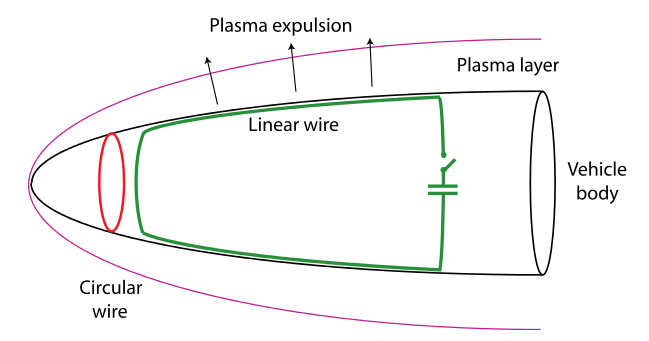
\includegraphics[width=0.5\textwidth]{Images/Stenzel_Implementation}
				\caption{\textbf{Potential implementation of the pulsed wire Lorentz window method, proposed by \cite{stenzel_new_2013}.}}
				\label{fig:Stenzel_Implementation}
			\end{figure}
			
			
			An alternate Lorentz window configuration uses the $\mathbf{E \times B}$ transport of electrons from an electric field induced by periodically rising current in a wire and the magnetic field induced by the wire current to create temporary regions of low plasma density which radiate outwards from the wire.\cite{stenzel_new_2013}
			
			Laboratory research done by Stenzel and Urrutia \cite{stenzel_new_2013} has shown that this technique could be plausible in creating temporary plasma windows.
			Figure \ref{fig:Stenzel_ExperimentConfig} shows the experimental configuration.
			
			Figure \ref{fig:Stenzel_ExperimentCurrentPlots} shows the results of the experimental work done by Stenzel and Urrutia.
			Saturation current of a Langmuir probe, which is proportional to the plasma density in that region of the plasma, initially peaks while the wire current increases, then gradually falls off before returning to normal after the wire current pulse has ended.
			
			Figure \ref{fig:Stenzel_ExperimentContourPlot} shows the plasma density expulsion from the wire during a current pulse.
			The low-density volume of plasma is preceded by a high density wave.
			The density front expands outwards radially from the wire loop above the ion plasma sound speed of $3\times10^5 cm/s$.\cite{stenzel_new_2013}
			
			The primary benefit of the pulsed Lorentz window technique is the simplicity of the implementation.
			Whereas a static $\mathbf{E\times B}$ field would require an electromagnet, the pulsed wire technique would simplify the hardware requirements.
			A possible implementation in a hypersonic vehicle is proposed by Stenzel and Urrutia in Figure \ref{fig:Stenzel_Implementation}.
			Pulsed currents through either the circular or linear wire would create radially propagating density waves in the plasma that could potentially be communicated through.

		\subsubsection*{Stokes Waves}
			Most active methods work by affecting the plasma and changing its properties, usually the plasma density, in order to make communication through the plasma more favorable.
			The Stokes wave method is unique in that it exploits the electromagnetic properties of the plasma itself to effectively use it as an antenna for both transmitting and receiving.
			Work done by Nazarenko et. al. and Korotkevich et. al. has established a plausible theoretical basis for the Stokes wave technique, though experimental verification is still necessary.\cite{nazarenko_communication_1994}\cite{korotkevich_communication_2007}
			
			To set up the process by which Stokes waves operate, we first briefly recall the propagation of electromagnetic waves in a plasma and the generation of Langmuir waves which was explored in section \ref{sec:Waves}.
			
			Consider an electromagnetic wave with frequency $\omega_0$ coming into contact with a one-dimensional plasma sheath with thickness $L$ and frequency $\omega_p$ at an angle $\theta$ with respect to the normal of the plasma surface, as shown in Figure \ref{fig:StokesDiagram}.
			From section \ref{sec:Waves}, we saw that if $\omega_0 \leq \omega_p$, the wave will be reflected by the plasma.
			Now consider a one-dimensional plasma with an electron number density given by $n(z)$, where $z$ is a spatial coordinate where the edge of the plasma is at $z=-L$, and the surface of the vehicle is at $z=R$.
			
			As the plasma density $n(z)$ increases traveling inwards towards the vehicle so does the cutoff frequency.
			The radio signal will travel into the plasma sheath until it reaches the point where $\omega_0 = \frac{\omega_p(z_r)}{Cos(\theta)}$.
			This is the reflection layer $z_r$ at which the electromagnetic wave will be reflected back towards its source.
			Oscillations induced in the plasma with frequency $\omega_0$ will continue to propagate as Langmuir waves, however, until they reach the resonance layer at $z=0$ where
			$\omega = \omega_p$, a large resonance in the electron oscillations occur.
			
			The goal of the Stokes wave technique is to bridge the gap between the surface of the vehicle and the electron oscillations in the resonance layer.
			The Stokes wave technique proposes using a process similar to Raman spectroscopy to scatter high-frequency electromagnetic waves off the resonance layer and collect the information from external electromagnetic waves which is encoded in the resonance layer.\cite{nazarenko_communication_1994}
			The returning wave that is scattered off the plasma resonance layer is called the Stokes wave.
			
			A ``pump" wave with frequency $\omega_{pm} > \omega_p$ is transmitted into the plasma sheath from the vehicle surface, where it interacts non-linearly with the oscillations in the resonance layer via Raman scattering.
			Most of the wave's energy will continue through the plasma, but a small amount will be scattered back towards the vehicle as a Stokes wave with frequency $\omega_s = \omega_{pm} - \omega_0$ carrying the information from the resonance layer.
			A separate receiver on the vehicle then receives the Stokes wave and decodes the information imprinted on it by the interactions in the resonance layer.
			In this way, the Stokes wave technique exploits the electromagnetic properties of the plasma sheath and effectively uses it as an antenna.
			
			The ratio of the electric field amplitude of the backscattered Stokes wave  $\left|\mathbf{E_s}\right|$ to the electric field amplitude of the signal wave $\left|\mathbf{E_t}\right|$ is given by
			\begin{equation}
			\label{eq:PowerLossRatio}
			\frac{\left|\mathbf{E_s}\right|}{\left|\mathbf{E_t}\right|} = \frac{eL\left|\mathbf{E_{pm}}\right|}{mc^2} \left(k_0 L\right)^{-1/3}
			\end{equation}
			A reasonable figure for this ratio is between 0.01 and 0.1, meaning that up to 10\% of the energy of the incident radio signal could be recovered as a Stokes wave by the vehicle.\cite{nazarenko_communication_1994}
			
			Perhaps the most appealing aspect of this technique is that the process is theoretically reversible for communicating outwards from the vehicle.
			In the vehicle-to-ground communication case, an analogous ``reverse" Stokes wave encodes the pump wave which induces oscillations in the plasma resonance layer.
			The oscillations in the resonance layer produce Langmuir waves which travel outwards and emit an electromagnetic wave with frequency $\omega_0 = \omega_{pm} - \omega_s$ carrying the information encoded by the Stokes wave.
			The resulting wave will have a similar power loss ratio to that given by equation (\ref{eq:PowerLossRatio}), however.
			Figure \ref{fig:StokesNumericalSim} shows a simulation done by the Korotkevich et. al. of a signal propagating through the plasma sheath from the vehicle.
			
			The Stokes wave method could potentially be limited by collisional damping in the plasma, non-uniformities of the plasma, and the short range of resonance for the resonance layer interactions.\cite{kim_electromagnetic_2009}
			Laboratory verification of this technique would be necessary for further analysis of its feasibility.
			
			\begin{figure}[t]
				\centering
				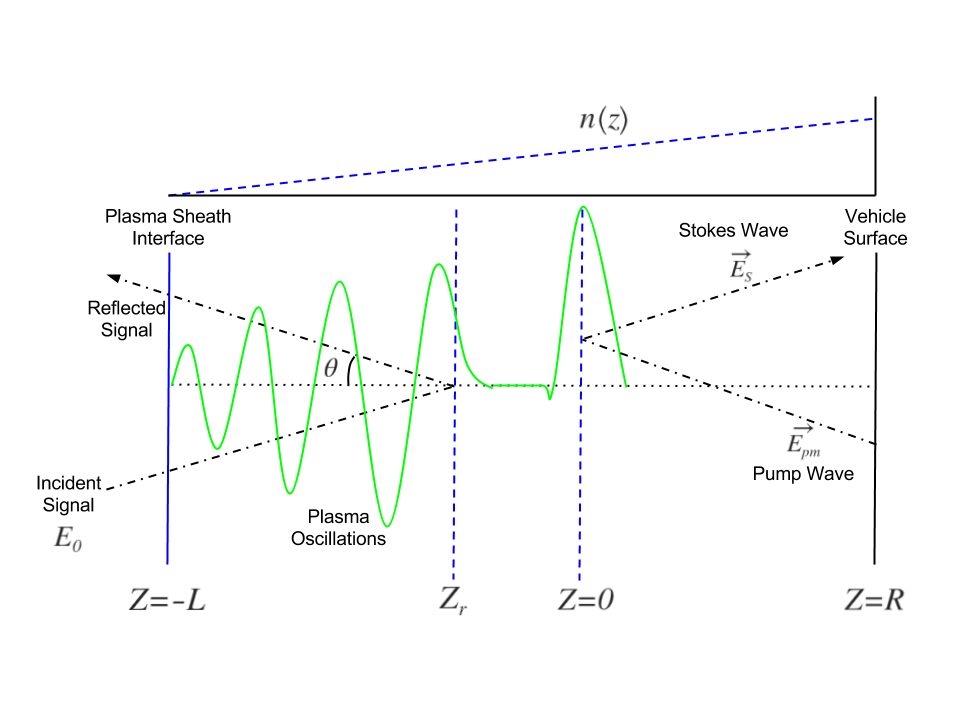
\includegraphics[width = 0.55\textwidth]{Images/StokesDiagram.png}
				\label{subfig:Stokes2}
				\caption{\textbf{A simplified 1D plasma sheath with density increasing from left to right with an incident signal wave from a ground station. The signal is reflected at $z_r$, but induced Langmuir oscillations continue to propagate forward into the plasma until the resonant layer at $z=0$ where $\omega_o = \omega_p(z=0)$.}}
				\label{fig:StokesDiagram}
			\end{figure}
			
			\begin{figure}[t]
				\centering
					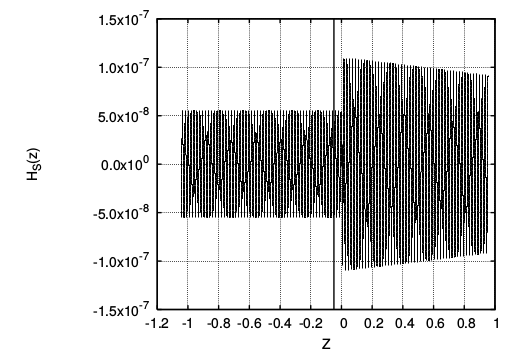
\includegraphics[width = 0.5\textwidth]{Images/Stokes_NumericalSim2.png}
					\label{subfig:Stokes2}
				\caption{\textbf{Numerical simulation of the magnetic field of a Stokes signal wave propagating from the vehicle to the resonance layer at $Z=0$ and being emitted as a lower-power signal.}}
				\label{fig:StokesNumericalSim}
			\end{figure}

\section*{Conclusion}
	The radio blackout problem arises when aircraft or spacecraft travel through an atmosphere at high hypersonic speeds, generating large volumes of dense plasma through aerodynamic heating which in turn block radio communications to or from the vehicle.
	The physics behind the radio blackout problem was examined in detail, including the role the plasma frequency $\omega_p$ plays in determining the cutoff frequency of radio waves propagating through the plasma.
	Various potential solutions that have been studied since the 1960's were looked at, including aerodynamic shaping, high frequency communication, liquid quenching, magnetic windows, lorentz windows, and Stokes waves.
	While each of these present a viable technical solution to the problem, solutions which minimize their overall effect on the vehicle's mass or performance and are simple to implement in general are highly preferable.
	Further laboratory analysis and flight testing in particular is required to determine the true feasibility of recent techniques such as Lorentz windows and Stokes waves.
\bibliographystyle{ieeetr}
\bibliography{plasma_blackout}


\end{document}
